In this work we define the chronological order assuming any possible combination of event assortment. We assume there is no golden order for any set of events when we hypothesise in terms of feasible outcomes.
\\

When discussing mutational events, the state-of-the-art discussion assumes an unordered system's biological dynamics. We hypothesise chronological order existence amongst the mutational events occurring within the cell.
\\

There are not sufficient backing studies to confirm order is in (or has) control of/over the full dynamics of the system. However, this work collects projects which have identified the impact order mutation events have on cancer progression. This fact serves as motivation to study conditions where conclusions on prognosis do not hold for every patient, and consider disease heterogeneity as an order-related issue.

\subsection{Gene mutation order impact on disease evolution}
\subsubsection{Number of events adding complexity}
In the cases of CRC \cite{Herbet2012AcquisitionPhenotypes} and the MPN studies \cite{Ortmann2015EffectNeoplasms}, two clearly differentiated condition evolution could be discerned by an order-based approach. A mere swap in the order of mutation of genes (\textit{ras} and \textit{p53}, and TET2 and JAK2, respectively) resulted in a less aggressive outcome for the patients. 
\\

Interestingly, the studies conclude the arrangement of pairs of mutational events as responsible for the outcome. These are always driver mutations relevant enough to dysregulate the full network they belong to when altered.

However, when including 4 events as in the second CRC study \cite{Fearon1990ATumorigenesis}, instead of setting a clear discriminatory factor among the sub-cases, the arrangement rather follows a \textit{frequency} approach, i.e. the order between events was established due to a majority of occurrences, despite having counterexamples. As we work with a larger number of alteration events, we would also expect a more complex system due to the known (and unknown) interactions among them. We could say the complexity of the conclusion would depend on the number of mutational events involved, although their nature (driver mutations, whole chromosomal loss, etc.) and consequences (dysregulation, blocking interaction, etc.) also weight in the final outcome.
\\

\begin{figure}
    \centering
    \begin{subfigure}[b]{0.5\textwidth}
      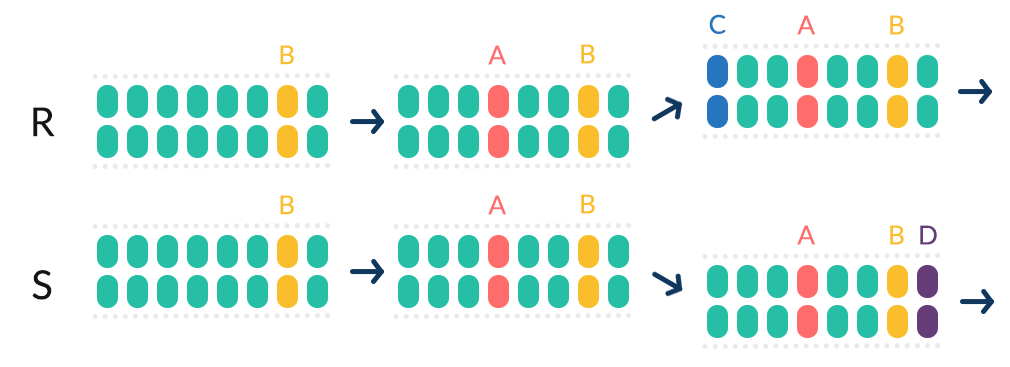
\includegraphics[width=\textwidth]{images/Div.png}
      \caption{Example of mutation divergence.}
      \label{fig:div}
    \end{subfigure}
    \hfill
    \begin{subfigure}[b]{0.40\textwidth}
      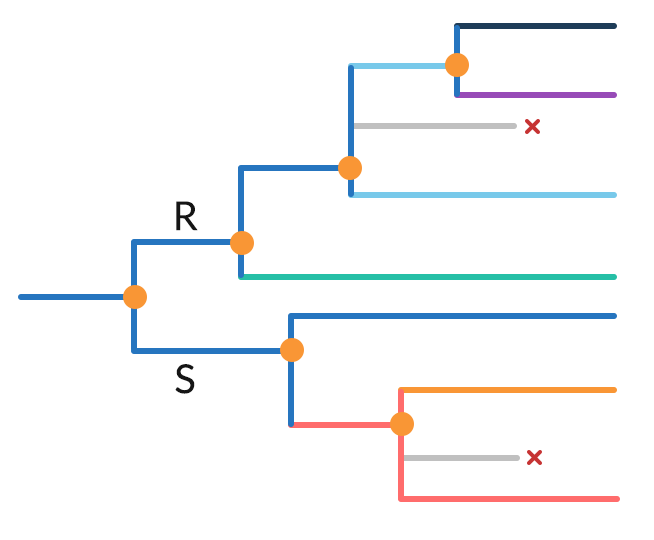
\includegraphics[width=\textwidth]{images/Pyl.png}
      \caption{Mutation evolution tree. Each colour represents a different clone. R and S branches from \ref{fig:div} are tagged too.}
      \label{fig:phyl}
    \end{subfigure}
    \caption{}
\end{figure}


\subsubsection{Building an event-evolution tree}
A possible explanation to the complexity might lay on the fact that a condition progress can have common steps in multiple individuals, but specific disrupting events can lead to a entirely divergent outcomes. Figure \ref{fig:div} shows a simple divergent effect in the mutation acquisition. If extended by considering all the alteration events of a case, it would result in an evolutionary tree whose in-between stages represent accumulated mutations on a timeline, and final states represent cell's final mutations (Figure \ref{fig:phyl}). This case would be the most highly detailed evolution followup of a condition, however its ramifications could be virtually exponential.
\\

The fact different order of occurrence amongst events result in that many different outcomes of the condition supports our hypothesis of chronological order. However, the supporting studies have reached cases where few (only 2 to 4) events can be highlighted.
\\

%Unleashing the applications
Assuming a scenario where order gains relevance, constituting chronological order then becomes the main challenge for the oncogenic field \cite{Gerstung2011TheTumorigenesis} based on the fact that clones can show vast clinical and histological differences, even when they share the same mutations. %Order's weight on the consequences also remains bound to environment and other circumstances such as inheritance, which is later discussed in this section.
\\

To simplify the hypothesis defence, I have assumed no other interaction interfere with the model, albeit the scenario is far from probable as cancer complexity cannot be studied leaving interaction out. Although clones might be lacking vital functions such as specific signal detection from external sources, the sub-clonal population is still present in the organism where the cancer developing, therefore this interaction must also be taken into consideration in a more complex study.

% GENERAL DISEASE HETEROGENEITY
% -------------------------------------------------
\subsubsection{Heterogeneity analysis}
Although the degree of discernment in other conditions remains largely unknown, heterogeneity within the clonal population could be analysed via phylogenetic trees analysis from which order can be retrieved.
\\

Based on the studies above, we know a full phylogenetic scenario displaying is challenging to retrieve, since the environment might contain a conglomerate of multiple divergent-evolved clones. Even so, many studies attempt to display the divergent scenario as accurately as possible  via phylogenetics \cite{Beerenwinkel2005Mtreemix:Trees} \cite{Rahnenfuhrer2005EstimatingScores}, or networks \cite{Hjelm2006NewOncogenesis} \cite{Gerstung2011TheTumorigenesis}. Mainly they aim at pinpointing events on a timeline that can later be used as support for tracing condition's evolution. Patient stratification becomes then a temporal issue\footnote{Defining a chronological system in which events are not strictly linear results in a branched scheme. Automata theory and Computational Tree Logic (CTL) model support this approach and offer good visualisations of the scenarios.} based on snapshots.
\\

It would also be a step forward in terms of heterogeneous clones eradication, which are the main issue when it comes to patient's relapse  \cite{Turajlic2016MetastasisProcess}.

% -------------------------------------------------
\subsubsection{Additional sources to support ordering}
Meta knowledge can be added to the study to aid chronological organisation as a reinforcement for ambiguous cases. E.g, based on TNM staging system, a clone starting node evasion is expected —although not limited to \cite{Turajlic2016MetastasisProcess}— in stage 4, therefore, effective driver mutations are expected later in the phylogenetic-tree-like model. Having a modest prediction of an event \textit{chronological belonging} could be highly indicative in terms of guiding the research. The method would be used to clear up ambiguities, not as the main principle of the procedure (this belongs to the pathway-based approach).
\\

Based on an evolutionary argument, there is also a \emph{weighting} effect on each mutation. Some driver mutations can be more harmful than others when it comes to consequences regarding behavior down the line. E.g. cell's apoptosis control system disruption generally initiates cancer. In terms of fitness, the more the progeny grows, the higher is the probability of alterations acquisition which enter the game of survival \cite{Gerstung2011TheTumorigenesis}. Therefore, correctly placing alterations driving apoptosis in a timeline should be tagged with a higher priority. Radical-stage inducing events such as apoptosis, cooperation loss, proliferation, metastasis, etc. would fall into the \textit{highly relevant} category.
\\

% -------------------------------------------------
\subsubsection{Clinical meaning and application}
Assuming historical order establishment, patient stratification and evolution prediction can rely on stage analysis. Chronological ordering of events offers a small grained display of the scenario. Then, tracing would be based on the timeline's evolution, and not on a single (current) snapshot obtained from samples 
\\

Pinpointing the exact stage of a cancer evolution having knowledge of past events leaves us with a highly sensitive model that helps us act on the most effective spot to break more lethal consequences.

Given the full spectrum of possibilities in which events can occur due to pure systems dynamics, the deductions and proposed lines of research can seem strict. However, they are not meant to solve the entire organisation by setting an order of mutations for each condition, but to offer discriminatory tools to use on cancer analysis and predictions.

% -------------------------------------------------
% PATHWAYS
% -------------------------------------------------
\subsection{Pathway disruption order impact on disease evolution}
%Drawbacks
Approaches based on pathways consider alteration events in a different way: If any member of the pathway's gene set is altered, this affects the full network which has any interaction with it. This mutation eventually triggers a cascade effect, disrupting all systems directly related to them. Therefore, looking at the problem from a more \textit{holistic} view, whose focus now is on setting order among pathways instead of genes, reduces complexity by generalising the cases.
\\

Making a sweeping assumption, properties inferred from gene-based models are conserved in pathway-based models in the following manner: pathway-based models first analyse individual gene mutations, and then map them to pathways. Then, any attribution or restriction bound to it (e.g. "belonging to an early stage" or "occurs before X mutation") will be transferred to the pathway it belongs to. Such transference needs a consensus regulation which controls how many evidences an inference would need to be accepted.
\\

%Strictness
In terms of restrictions, stronger evidence for order constraints in pathways than in gene level order is no surprise, since pathway-driven approaches consider whole systems whose dysregulation is only noticeable when it largely ceases to work (full pathway disruption), while gene-based methods reflect rapid, although small-range changes.

%Cannot rely only on frequency
Studies like \cite{Cheng2012AGliomagenesis} use a hybrid method for order establishment. Via cross-correlation analysis alone, the inference can only order 2 pathways before ambiguities arise. The uncertainties are then solved using \emph{in vitro} assays to enhance the available samples. It is probable that not all the stages of the cancer evolution are present in the samples, which opens a void in the available knowledge.

% Cycle speed
Frequency thresholds act as a filter for samples which are truly significant, but not frequent enough to be taken into consideration (Figure \ref{fig:mlink}). A specific Missing-Link (mLink) case recurrence is then proportional to the clone's fitness, i.e. the less we find a cell (potential mLink) in a sample, the more probable is other populations have won the survival race and replaced it. It is also bound to cell's cycle speed that transition from pre-mLink to post-mLink through mLink itself could have happened in a time period insufficient for its measurement.

Filling the gap with more evidence is necessary in order to avoid the assortment to remain incomplete.

\begin{figure}[!ht]
    \centering
    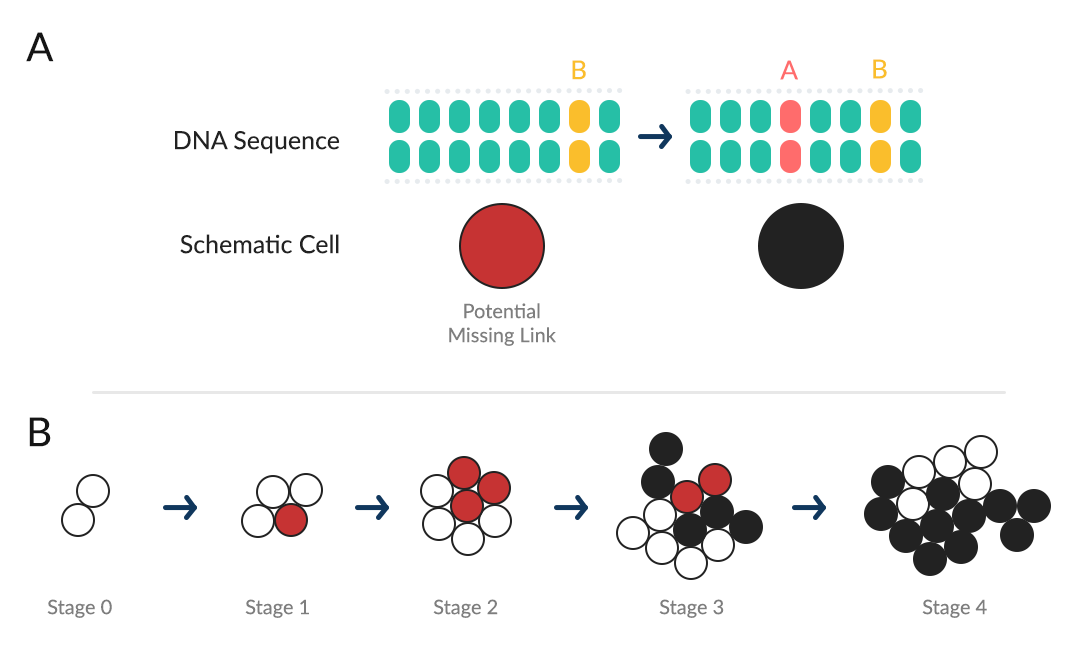
\includegraphics[width=\linewidth]{images/Mlink.png}
    \caption{Missing link hypothesis: (A) Cancerous cells displaying different mutations. The simplified red cell evolves to the simplified black cell. (B) Displays how a clonal population might evolve. The red cells are the forerunners of the black ones, and the latter end up outnumbering the parent cell. Such scenario leaves a missing link in order inference based on frequency analysis.}
    \label{fig:mlink}
\end{figure}


\subsubsection{Future hypothesis: Hallmarks of order-driven approaches}
%First: Progression, prognosis and survival.
Being able to identify several subtypes within a cancer introduces two hallmarks: First, specific subtype tracing and analysis can confer us further insight about survival. Although the general lines of cancer progression follow the same line within a cancer type, each subtype has a unique set of characteristics (e.g. Breast Cancer). Via in-depth pathway analysis, a similar evolutionary tree as in Figure \ref{fig:phyl} could be built for pathways, and classify current histologic, genetic, and prognostically heterogeneous cases in more specific subtypes (e.g. triple-negative Breast Cancer).

Besides, the fact of knowing which point of the chronology is expected to be dysregulated next or actionable in the following step sets a huge advantage in treatment.
\\

%Second: Relative importance
The second hallmark is derived from subtype analysis, focusing on its progression. Based on the consequences, relative relevance can be assigned to driver mutations, e.g. RB and TP53 pathways are related to early stages of oncogenesis because their alteration interferes with normal cell cycle and growth, hence, these events hold a higher priority.
\\

\subsection{Inheritance implications in the picture}
According to American Society of Clinical Oncology (ASCO) \footnote{\url{https://www.cancer.net}}, cancer caused by germline mutations accounts for about 5\%-20\% of all cancers.
\\

Studies like \cite{DeLaChapelle2004GeneticCancer} are indicative of how the predisposition is relevant in diverse cancer subtypes. For each condition, the genetic baggage supposes a different starting point (Figure \ref{fig:inh}), then, any \textit{expected} order of alterations could not be met.

\begin{figure}[!hb]
    \centering
    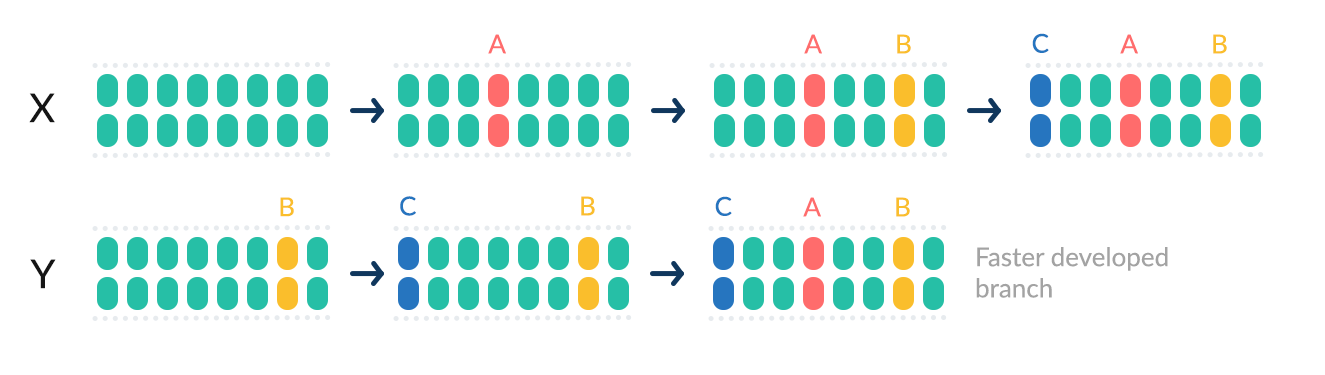
\includegraphics[width=\linewidth]{images/NInN.png}
    \caption{ypothesis of inheritance impact on ordered events. (X) shows an assumed regular order A $\rightarrow$ B $\rightarrow$ C. Then, (Y) represents inheritance of the B mutation, which results in a different inference of order: B $\rightarrow$ C $\rightarrow$ A.}
    \label{fig:inh}
\end{figure}


Since in they can accelerate the pace at which cancer starts and evolves, the relative relevance of events also gets blurred. A previously low-ranked alteration event (e.g. because its appearance was expected at a late stage) might gain now interest as its accumulation to other mutations implies a progress in the condition.

All in all, based on the knowledge we have on germline-related study, and also being aware of the lack of a link between gene/pathway chronological order and inheritance significance and impact on its onset, we hypothesise inherited mutations do have an impact on event order in that they clutter the techniques used to accurately establish an assortment. On contrast, somatic alterations are the main \emph{natural} course we'd expect for order decoding, then they can be considered as less detrimental for the order-based approaches.